\chapter{Introdução} \label{introducao}



\section{Contextualização} \label{contextualização}

A evolução das comunicações, desde o seu início em 1980 com a primeira geração (1G) até os dias de hoje, vem sendo pautada na implementação de melhorias a um sistema anterior. A segunda geração (2G) deu início a era digital, que buscava corrigir a questão de segurança da rede analógica. A terceira geração (3G) surgiu para permitir o tráfego de dados, que existia na 2G de forma muito tímida. A quarta geração (4G), por sua vez, foi desenvolvida para aumentar a qualidade de serviço, resolvendo problemas como instabilidade e baixa velocidade de tráfego \cite{Best}. 
\par A próxima geração (5G) vem para quebrar paradigmas. Os problemas atuais não demandariam uma nova geração de telefonia para serem corrigidos. Tratam-se de questões relacionadas a cobertura e custo, que não requerem novos padrões ou funcionalidades. Entretanto, a estagnação na 4G poderia limitar o desenvolvimento de diversas tecnologias e buscando evitar isso, a 5G tenta construir padrões que permitirão às sociedades futuras uma realidade muito diferente da atual.
\par Nesse contexto, fala-se em uma divisão da geração futura em três categorias: \textit{enhanced mobile broadband (eMBB)}, que procura melhorar a comunicação móvel de banda larga; \textit{machine-type communications (mMTC)}, que desenvolve a comunicação dispositivo a dispositivo (D2D) e \textit{ultra reliable MTC (uMTC)}, que deseja confiabilidade na comunicação entre máquinas [\cite{Qualcomm}]. A ideia é desenvolver cada uma dessas categorias de forma a viabilizar, entre outras aplicações \cite{Wunder}

\begin{enumerate}
\item \textbf{internet das coisas} (IoT \textit{Internet of Things})  
\item \textbf{conectividade sem fios a uma velocidade de Gigabits/s}
\item \textbf{internet tátil}
\end{enumerate} 

A IoT é algo grandioso. Imagina-se a conexão massiva entre dispositivos, veículos, sensores - realmente "coisas". Ao contrário do que se observa hoje, não serão mais as pessoas as dominadoras do tráfego de dados, mas sim os objetos. A internet das coisas poderá trazer um sem número de benefícios, como se observa em estudos de aplicação desse conceito: \cite{Prouski} \cite{Saha} \cite{Hlaing}. 
\par Essas propostas não são realizáveis a baixas velocidades. Deve-se lembrar, ainda, que mesmo sem a \textit{IoT}, o tráfego de dados convencionais tem crescido de forma expressiva e que os usuários da modalidade tem se tornado cada vez mais exigentes quanto à qualidade de serviço (QoS) e à velocidade de navegação. É nesse contexto que a segunda aplicação aparece, com avidez pela transmissão rápida de dados; na verdade, tão veloz que se compararia ao que hoje só se experimenta quando da conexão por fios. 
\par A internet tátil também corrobora o desejo por agilidade. Ela engloba as aplicações de tempo real, como as exemplificadas em \cite{Fettweis1}. Além do requisito de celeridade, é impeditivo trabalhar com atrasos, o que diminui a ordem de tolerância a latência aos $\mu$s. 
\par Percebe-se que tornar o 5G uma realidade é, sem dúvidas um desafio. As atividades anteriormente mencionadas modificarão de manteira drástica a arquitetura de rede atual, como mostram as figura \ref{Figura_arquitetura_atual}. 

\begin{figure}[h!]
\centering
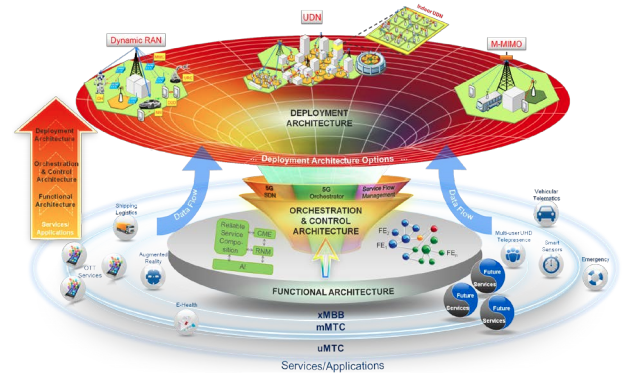
\includegraphics[width=3.5in]{Figura_arquitetura}
\caption{Arquitetura 5G \cite{MetisD28}}
\label{Figura_arquitetura_atual}
\end{figure}

Incrivelmente, a forma de onda OFDM (\textit{Orthogonal Frequency Division Multiplexing}), que foi a grande possibilitadora da 4G, pode representar um obstáculo a essa nova fase. Os requisitos de ortogonalidade e sincronismo do OFDM não conversam com as soluções imaginadas para tornar a quinta geração possível \cite{Wunder}. 

\par O problema começa com o tráfego esporádico (TE) \cite{Wild}, demandado pela IoT. Os dispositivos não estarão em comunicação com a rede continuamente. Isso é impraticável a equipamentos alimentados por baterias, por ser totalmente ineficiente do ponto de vista energético. A ideia é simples: se o equipamento possui uma mensagem ele se conecta a rede, entrega sua informação e se desconecta. Para que isso funcione com os requisitos LTE de sincronismo, seria necessário acoplar ao sinal transmitido uma considerável parte dedicada a controle, o que representa um desperdício de recurso \cite{Wunder}. Essa dificuldade já é evidenciada hoje, no \textit{fast dormancy} \cite{Zhao}, mecanismo utilizado por fabricantes de celulares.    
\par O sincronismo se mostra como um empecilho mais uma vez quando esbarra na ideia de cooperação entre células adjacentes (CoMP) \cite{Wunder}. Este conceito é utilizado na 4G e melhora o desempenho do sistema a medida que combina diferentes antenas para transmissão e recepção, ainda que estas não estejam na mesma célula \cite{DLee}. Se para enviar mensagens sem contato simultâneo com a rede já se demanda uma quantidade considerável de bits de uma mensagem dedicada a sinals de controle, para sincronizar várias BSs e estações móveis (MSs), o cenário é muito pior. Ainda, os sinais recebidos por cada MS sofrem atrasos diferentes a depender da estação que os emite. Isto, somado ao atraso natural de qualquer canal sem fio, exigiria um prefixo cíclico muito grande nos caso de símbolos OFDM para que a interferência fosse mitigada, contribuindo ainda mais pro \textit{overhead} do símbolo em transmissão \cite{Wunder}. 
\par A esses reveses, apresenta-se como solução a utilização de uma nova forma de onda na camada físca (PHY) 5G, a qual não tenha como característica fundamental a ortogonalidade e o sincronismo. Em seu lugar, sugere-se a utilização de filtros como instrumento de mitigação de interferências, os quais podem ser aplicados a cada subportadora, como propõe o FBMC (Filter Bank Multicarrier); ou a sub-bandas, cujo número de subportadoras filtradas em conjunto pode variar - proposta do UFMC (Universal Filtered Multicarrier). 
\par A próxima seção trata das considerações ao se utilizar uma nova forma de onda e mostra porque este tema foi escolhido para ser explorado neste trabalho. 

\section{Descrição do Problema e Contribuição do Trabalho}
 
Na seção \ref{contextualização}, mostrou-se que o uso de novas formas de onda na camada PHY é um grande passo na viabilização das novas aplicações previstas para a 5G. Torna-se, então, importante confirmar que podemos tratá-las como uma alternativa. É por isso que, tanto na academia \cite{Liu}, \cite{Gerzaguet} quanto na indústria, existe uma mobilização em testar essas candidatas, seja em termos de sua complexidade de implementação, seja em relação ao seu desempenho em alguns cenários típicos às comunicações móveis.  
\par Este trabalho busca explorar o tema especificamente em relação a resposta dessas formas de onda quando submetidas a efeitos não lineares, um tipo de imperfeição usual em canais de radio frequência (RF). Sistemas de telecomunicação sem fio apontam para a necessidade de uso amplificadores de potência, que costumam gerar este tipo de distorção.  
\par A literatura já apresenta alguns resultados comparativos do OFDM às formas de onda principais, FBMC e UFMC \cite{Changyoung},\cite{Maheswari} , mas ainda está evoluindo na proposição de sistemas de correção. É nesta direção que se move este trabalho e pode-se resumir suas contribuições aos tópicos a seguir:
\begin{itemize}

\item compilação de análises comparativas prévias em relação ao desempenho das principais formas de onda candidatas a 5G,
\item avaliação do desempenho dessas formas de onda quando submetidas às não-linearidades para dois cenários: um que considera e outro que descarta os efeitos de memória
\item proposição de um algortimo de correção iterativa, o ICHD (\textit{iterative correction with hard detection}), que ainda não havia sido aplicado a 5G e
\item avaliação de efetividade da aplicação do algoritmo de pre-distorção digital (DPD) as ondas candidatas quando os efeitos de memória são levados em consideração. 
 
 \end{itemize}

